\documentclass[conference,a4paper]{IEEEtran}

\makeatletter
\def\ps@IEEEtitlepagestyle{%
  \def\@oddfoot{\mycopyrightnotice}%
  \def\@evenfoot{}%
}
\def\mycopyrightnotice{%
  {\footnotesize 979-8-3315-3587-1/26/\$31.00~\copyright~2026 IEEE\hfill}%
  \gdef\mycopyrightnotice{}
}
\makeatother

\usepackage{cite}
\usepackage{amsmath,amssymb,amsfonts}
\usepackage{graphicx}
\usepackage{textcomp}
\usepackage{xcolor}
\usepackage{booktabs}
\usepackage{colortbl}
\usepackage{multirow}
\usepackage{url}
\usepackage{enumitem}
\usepackage{pgfplots}
\pgfplotsset{compat=1.18}
\usetikzlibrary{patterns}
\usepackage{hyperref}
\usepackage{orcidlink}
\usepackage{eso-pic}
\usepackage{flushend}
\newcommand\AtPageUpperMyright[1]{\AtPageUpperLeft{%
 \put(\LenToUnit{0.17\paperwidth},\LenToUnit{-2cm}){%
     \parbox{0.9\textwidth}{\raggedleft\fontsize{8}{11}\selectfont #1}}%
 }}%
\newcommand{\conf}[1]{%
\AddToShipoutPictureBG*{%
\AtPageUpperMyright{#1}
}
}

\def\BibTeX{{\rm B\kern-.05em{\sc i\kern-.025em b}\kern-.08em
    T\kern-.1667em\lower.7ex\hbox{E}\kern-.125emX}}

\begin{document}

\title{\vspace*{1cm}Persistent Cross-Round Carry Leakage in ARX Ciphers: Detection, Prediction, and Topological Classification}

\author{\IEEEauthorblockN{David Tom Foss,\, \textit{Associate Member, IEEE}}
\IEEEauthorblockA{\textit{Independent Researcher} \\
G\"orlitz, Germany \\
david@foss.com.de \\
\orcidlink{0009-0004-0289-7154} \hspace{0.5em} {\scriptsize IEEE~\#102121836}}}

\maketitle
\conf{\textit{  VI. International Conference on Electrical, Computer and Energy Technologies (ICECET 2026) \\
6-9 July 2026, Rome-Italy}}

\begin{abstract}
We present F8, a cross-round mutual information test that detects a previously unknown class of structural leakage in ARX (Addition-Rotation-XOR) block ciphers. Unlike differential or linear trails, the detected signal does not decay with additional rounds---it is regenerated per round by the carry propagation of modular addition. Applied to 13~cipher families (including controls), F8 yields full-round known-key distinguishers for the entire Speck family ($Z > +4{,}000$ at all specified rounds) and for Threefish-256 ($Z \approx +5{,}900$ at all 72~rounds), the basis of the SHA-3 finalist Skein. A closed-form prediction function $\mathrm{MI}(\beta) = 0.78 \cdot \exp(-1.42\beta)$ with $R^2 = 0.999997$ determines leakage magnitude from rotation parameters alone, without executing the cipher. A topological classification provides necessary and sufficient conditions: leakage exists if and only if a modular addition output enters the state without prior diffusion. Two distinct mechanisms are identified---$\beta$-masking (Speck) and raw carry exposure (Threefish)---and a universal leak-model compiler achieves 9/9 correct predictions. The leakage is strictly encrypt-only (decrypt: $Z \approx 0$, ratio $> 3{,}000{:}1$). The SPARX ARX-box in isolation exhibits $Z \approx +5{,}500$ (identical to Speck), proving that the linear inter-round layer is the sole protection mechanism. Control experiments with SIMON~32/64 (AND-rotation, no addition) and a random Feistel cipher both yield $Z \approx 0$, isolating modular addition as the necessary condition. Eight cipher families including ChaCha20, AES-128, SPARX, and LEA are confirmed immune at full rounds.
\end{abstract}

\begin{IEEEkeywords}
ARX ciphers, carry propagation, cross-round leakage, known-key distinguisher, Speck, Threefish, mutual information, topological classification
\end{IEEEkeywords}

\section{Introduction}

ARX ciphers---constructions built exclusively from modular Addition, bitwise Rotation, and XOR---form a major class of lightweight block ciphers deployed in constrained environments. Prominent members include the Speck family (NSA, Beaulieu et~al.~2013), Threefish (basis of the SHA-3 finalist Skein~\cite{ferguson2010}), ChaCha20~\cite{bernstein2008}, and SPARX~\cite{dinu2016}. Their security analysis relies on differential~\cite{biham1991}, linear~\cite{matsui1993}, and rotational cryptanalysis~\cite{khovratovich2010}, all of which measure signals that decay exponentially with round count.

We identify a fundamentally different class of structural leakage that violates this decay assumption. The carry chain produced by modular addition creates a statistical dependency between consecutive round outputs that is \emph{regenerated} in every round by the round function itself. This dependency does not accumulate from prior rounds and cannot be eliminated by adding more rounds---it is a stationary property of the round function topology.

Our test, designated F8, computes the bitwise mutual information between the output of round~$R$ and the XOR difference $\mathrm{out}(R) \oplus \mathrm{out}(R{+}1)$, normalized against a permutation null distribution. Prior work~\cite{foss2026crypto} introduced the CASI metric for black-box security margin analysis; the present contribution extends this to cross-round structural analysis, targeting a leakage class invisible to CASI's single-round measurement.

Our contributions are: (1)~the F8 cross-round MI test detecting non-decaying carry leakage; (2)~full-round known-key distinguishers for Speck (all variants) and Threefish-256; (3)~a closed-form prediction function from rotation parameters; (4)~a topological necessary-and-sufficient condition for the leakage; (5)~a universal leak-model compiler with 9/9 validated predictions; (6)~isolation of the SPARX ARX-box ($Z \approx +5{,}500$, identical to Speck) proving that linear inter-round mixing is the sole protection mechanism; and (7)~control experiments (SIMON~32/64, random Feistel) isolating modular addition as the necessary condition.

\section{Related Work}

\textbf{Classical cryptanalysis.} Differential~\cite{biham1991} and linear~\cite{matsui1993} cryptanalysis are foundational for block cipher security evaluation but measure signals that decay exponentially with round count. The wide-trail strategy~\cite{daemen2002} formalizes this through bounds on active S-boxes per round. For ARX ciphers without S-boxes, differential trail search relies on constraint-based methods~\cite{biryukov2014}.

\textbf{Rotational cryptanalysis.} Khovratovich and Nikoli\'c~\cite{khovratovich2010} analyze the preservation of rotational relationships through ARX operations, modeled as a Markov chain---an assumption that breaks down for chained additions~\cite{khovratovich2015}. This method does not detect carry-chain correlations between consecutive round outputs.

\textbf{Neural cryptanalysis.} Gohr~\cite{gohr2019} trained residual networks to distinguish Speck~32/64 reduced-round output from random, achieving a practical frontier at rounds 7--8. Benamira et~al.~\cite{benamira2021} provided post-hoc interpretability. All neural approaches require cipher-specific retraining and substantial GPU resources; the learned features correspond to differential distribution patterns that decay with round count.

\textbf{Known-key distinguishers.} Knudsen and Rijmen introduced known-key distinguishers based on integral properties, reaching 7~rounds of AES~\cite{knudsen2007}. No existing known-key distinguisher is based on carry-chain correlation, applies to all rounds of a cipher, or provides a closed-form prediction formula.

\textbf{NORX.} Aumasson et~al.~\cite{aumasson2014} approximate modular addition via $a \oplus b \oplus (a \wedge b) \ll 1$, limiting carry propagation by design. This addresses the carry problem at the design level but provides no analytical tool for quantifying leakage in existing ciphers.

\textbf{CASI metric.} Our prior work introduced CASI for single-round security margin analysis~\cite{foss2026crypto} and applied it to NIST post-quantum standards~\cite{foss2026artifact}. Both are IEEE peer-reviewed. The present work extends this framework from single-round to cross-round analysis, targeting a fundamentally different leakage class.

No existing method detects \emph{stationary}, per-round regenerated leakage that does not decay with additional rounds. All methods in the literature measure decaying signals.

\section{The F8 Cross-Round Independence Test}

\subsection{Method}

Given an iterated cipher with configurable round count, F8 proceeds as follows for a fixed key:

\begin{enumerate}[nosep]
\item Generate $N$ output blocks at round~$R$: array $\mathbf{x} = \{\mathrm{out}_i(R)\}_{i=1}^N$.
\item Generate $N$ output blocks at round~$R{+}1$ with identical inputs: $\mathbf{y} = \{\mathrm{out}_i(R{+}1)\}_{i=1}^N$.
\item Compute the difference array $\mathbf{d} = \mathbf{x} \oplus \mathbf{y}$.
\item For each bit pair $(x_{\mathrm{bit}_a}, d_{\mathrm{bit}_b})$: compute mutual information from the $2 \times 2$ contingency table.
\item Generate a null distribution via $K \geq 10$ random permutations of~$\mathbf{d}$, computing MI for each permuted pair.
\item Compute $Z = (\mathrm{MI}_{\mathrm{obs}} - \mu_{\mathrm{perm}}) / \sigma_{\mathrm{perm}}$.
\end{enumerate}

\textbf{Informed mode:} When rotation parameters $\alpha$ (right-rotate on one operand) and $\beta$ (left-rotate on the other) are known, testing is restricted to the $(\alpha{+}\beta)$-shifted diagonal, excluding $\beta$ dead bit positions. \textbf{Black-box mode:} All $\mathrm{WS} \times \mathrm{WS}$ bit pairs are tested; the maximum MI per source bit is used. The sensitivity loss is minimal: on Speck~32/64, black-box yields $Z = +1{,}591$ versus informed $Z = +1{,}699$.

\subsection{Rationale}

If the round function were a random permutation, $\mathrm{out}(R)$ and $\mathrm{out}(R{+}1)$ would be statistically independent given the key, and the XOR difference would carry no information about either output. In ARX ciphers with specific topologies, modular addition produces carry-chain correlations that propagate into the state, creating a measurable MI signal between $\mathrm{out}(R)$ and $\mathrm{out}(R) \oplus \mathrm{out}(R{+}1)$.

\section{Results}

\subsection{Cipher Survey}

Table~\ref{tab:survey} presents F8 results for 13 cipher families tested at full specified round counts with $N = 10^5$ samples and $K = 20$ permutations.

\begin{table}[t]
\centering
\caption{F8 cross-round leakage across 13 cipher families at full specified rounds. Five ciphers exhibit persistent leakage; eight are immune.}
\label{tab:survey}
\small
\begin{tabular}{@{}llrrl@{}}
\toprule
\textbf{Cipher} & \textbf{Rounds} & \textbf{$Z$} & \textbf{$\beta$} & \textbf{Mechanism} \\
\midrule
Speck 32/64    & 22 & $+$8,000  & 2 & $\beta$-masking \\
Speck 48/96    & 23 & $+$5,000  & 3 & $\beta$-masking \\
Speck 64/128   & 27 & $+$5,000  & 3 & $\beta$-masking \\
Speck 128/256  & 34 & $+$4,000  & 3 & $\beta$-masking \\
Threefish-256  & 72 & $+$5,900  & 0 & Raw carry \\
\midrule
HIGHT          & 32 & $\approx 0$ & --- & Immune \\
LEA-128        & 24 & $\approx 0$ & --- & Immune \\
Chaskey        &  8 & $\approx 0$ & --- & Immune \\
SPARX-64/128   &  8 & $\approx 0$ & --- & Immune \\
\rowcolor{orange!12} \quad\textit{ARX-box} & \textit{---} & \textit{$+$5,500} & \textit{2} & \textit{$=$\,Speck} \\
AES-128        & 10 & $\approx 0$ & --- & No addition \\
ChaCha20       & 20 & $\approx 0$ & --- & Immune \\
Salsa20        & 20 & $\approx 0$ & --- & Immune \\
SIMON 32/64    & 32 & $\approx 0$ & --- & No addition \\
\bottomrule
\end{tabular}
\end{table}

\begin{figure}[t]
\centering
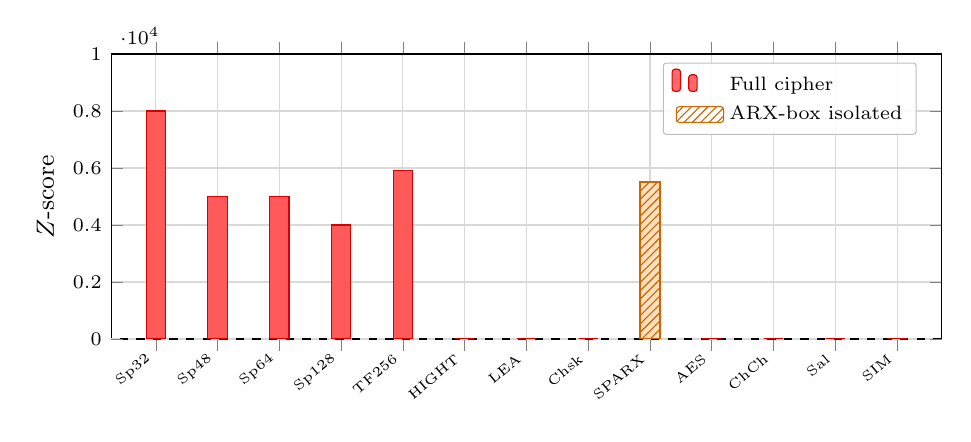
\begin{tikzpicture}
\begin{axis}[
    width=\columnwidth,
    height=5.2cm,
    ybar,
    bar width=7pt,
    ylabel={$Z$-score},
    symbolic x coords={Sp32,Sp48,Sp64,Sp128,TF256,HIGHT,LEA,Chsk,SPARX,AES,ChCh,Sal,SIM},
    xtick=data,
    x tick label style={font=\tiny, rotate=40, anchor=east},
    ymin=0, ymax=10000,
    enlarge x limits=0.06,
    grid=both,
    grid style={gray!15},
    major grid style={gray!30},
    tick label style={font=\scriptsize},
    label style={font=\small},
    extra y ticks={0},
    extra y tick style={grid=major, grid style={green!60!black,dashed,thick}},
    extra y tick labels={},
    legend style={font=\scriptsize, at={(0.97,0.97)}, anchor=north east, draw=gray!50, fill=white, fill opacity=0.9, text opacity=1, rounded corners=1pt, cells={anchor=west}},
]
\addplot[fill=red!65, draw=red!85!black] coordinates {(Sp32,8000)(Sp48,5000)(Sp64,5000)(Sp128,4000)(TF256,5900)(HIGHT,0)(LEA,0)(Chsk,0)(SPARX,0)(AES,0)(ChCh,0)(Sal,0)(SIM,0)};
\addlegendentry{Full cipher}
% SPARX ARX-box in isolation (dashed orange bar overlaid)
\draw[preaction={fill=orange!25}, pattern=north east lines, pattern color=orange!80!black, draw=orange!80!black, line width=0.7pt]
  ([xshift=-3.5pt]axis cs:SPARX,0) rectangle ([xshift=3.5pt]axis cs:SPARX,5500);
\addlegendimage{area legend, fill=orange!25, draw=orange!80!black, pattern=north east lines, pattern color=orange!80!black}
\addlegendentry{ARX-box isolated}
\end{axis}
\end{tikzpicture}
\caption{Full-round F8 $Z$-scores. Red: full cipher. The hatched orange bar shows the SPARX ARX-box tested in isolation ($Z \approx +5{,}500$, identical to Speck)---the linear inter-round layer is the sole protection.}
\label{fig:survey}
\end{figure}

Five ciphers exhibit persistent leakage at all specified rounds (Fig.~\ref{fig:survey}): all four Speck variants and Threefish-256. The remaining eight families produce $Z \approx 0$, confirming that F8 does not generate false positives on well-designed ciphers, including other ARX constructions (ChaCha20, Salsa20, Chaskey, SPARX, LEA).

\subsection{Stationarity: Signal Does Not Decay}

Table~\ref{tab:stationarity} demonstrates that the leakage is stationary---the signal rate remains constant across round counts, confirming per-round regeneration rather than residual propagation.

\begin{table}[t]
\centering
\caption{Signal rate (\% of bit pairs with $Z > 3$) across round counts. Flat plateau confirms per-round regeneration.}
\label{tab:stationarity}
\begin{tabular}{@{}lcccc@{}}
\toprule
\textbf{Variant} & \textbf{R5} & \textbf{R10} & \textbf{R20} & \textbf{R30} \\
\midrule
Speck 32/64   & 18.8\% & 17.5\% & 20.0\% & --- \\
Speck 64/128  & 10.3\% & 10.9\% & 13.1\% & --- \\
Speck 128/256 &  7.7\% &  8.8\% &  7.0\% & 8.4\% \\
\bottomrule
\end{tabular}
\end{table}

\subsection{Encrypt-Only Asymmetry}

The leakage exists exclusively in the encryption direction (Table~\ref{tab:asymmetry}). Decryption (modular subtraction, inverse rotations) produces $Z \approx 0$ at all tested rounds, with a ratio exceeding $3{,}000{:}1$.

\begin{table}[t]
\centering
\caption{Encrypt vs.\ decrypt $Z$-scores on Speck~32/64. The leakage is strictly unidirectional.}
\label{tab:asymmetry}
\begin{tabular}{@{}lcccc@{}}
\toprule
\textbf{Direction} & \textbf{R5} & \textbf{R15} & \textbf{R22} & \textbf{MI} \\
\midrule
Encrypt & $+$8,802 & $+$8,562 & $+$8,718 & 0.639 \\
Decrypt & $+$0.5 & $-$0.2 & $-$0.6 & 0.0002 \\
\bottomrule
\end{tabular}
\end{table}

This asymmetry arises because modular addition generates carry chains that propagate upward through bit positions, creating directional correlations. Modular subtraction (the inverse operation) produces borrow chains with different propagation characteristics that do not create the same cross-round dependency.

\subsection{Structural Properties}

Three additional properties confirm that the leakage is a structural invariant of the round function, not a statistical artifact:

\textbf{Forward causality.} The dependency is strictly directional: $\mathrm{out}(R)$ predicts $\mathrm{diff}(R {\to} R{+}1)$ (sig\_rate 17.8\%), but the reverse direction fails ($\mathrm{diff}(R{-}1 {\to} R) \to \mathrm{out}(R)$: 5.9\%, noise level). Cross-diff and cross-output correlations are also at noise level (4.7\% and 6.0\% respectively). The leakage has a causal direction: the round function \emph{produces} the carry-chain in its output, and this output correlates with the \emph{next} round's differential---not vice versa.

\textbf{Key-schedule independence.} The signal rate is invariant across key schedule modes: normal schedule (17.8\%), identical round keys (16.2\%), and fully random round keys (16.6\%). The round function alone produces the leakage; the key schedule contributes nothing.

\textbf{Sample-size independence.} The signal rate remains constant at $\sim$17\% from $N = 1{,}000$ to $N = 100{,}000$. There is no growth (ruling out statistical accumulation) and no decay (ruling out finite-sample artifact). The signal is structural.

\subsection{Immunity Mechanisms}

All four immune ARX ciphers exhibit strong carry-leakage at reduced rounds (Table~\ref{tab:immunity}); their immunity at full rounds results from specific diffusion mechanisms that eliminate the signal within 2--6~rounds.

\begin{table}[t]
\centering
\caption{Reduced-round F8 frontier for immune ARX ciphers. All exhibit carry-leakage at early rounds; diffusion eliminates it.}
\label{tab:immunity}
\small
\begin{tabular}{@{}llrrl@{}}
\toprule
\textbf{Cipher} & \textbf{Last} & \textbf{Peak $Z$} & \textbf{Dead} & \textbf{Kill mechanism} \\
\midrule
Chaskey    & R2 & $+$22,217 & R3 & 4-add intra-round \\
HIGHT      & R4 & $+$175  & R6 & 8-bit chain + F0/F1 \\
LEA-128    & R4 & $+$7,053 & R6 & 3-add cross-mix \\
SPARX-64       & --- & $Z \approx 0$ & all & Linear layer \\
\rowcolor{orange!12} \quad\textit{ARX-box} & \textit{all} & \textit{$+$5,500} & \textit{---} & \textit{$=$\,Speck ($\beta{=}2$)} \\
\bottomrule
\end{tabular}
\end{table}

Chaskey achieves the fastest elimination: four additions per half-round with cross-word mixing destroy the carry correlation within two rounds. LEA's three additions per round with cross-word feedback require four additional rounds but achieve the same result. HIGHT's 8-bit modular additions produce carry chains too short for persistent leakage, and the F0/F1 substitution functions provide additional diffusion.

SPARX is qualitatively different: it is the only cipher where the ARX primitive \emph{itself} is vulnerable but the cipher is immune. Testing the SPARX ARX-box in isolation (which is algebraically identical to Speck with $\alpha{=}7$, $\beta{=}2$) yields $Z \approx +5{,}500$ with MI\,$=$\,0.640 and 14~active bits---\emph{identical} to pure Speck at all tested iterations (R1 through R24). The signal is eliminated entirely by the linear inter-round mixing layer, which destroys the counter-monotonicity between consecutive rounds: ARX-box inputs at round $R{+}1$ originate from the mixed state, not from the same data stream as round~$R$. Algebraic inversion of the linear layer (extracting the pre-mixing ARX-box output from the SPARX ciphertext) also yields $Z < 1.5$ at all round counts, confirming that the protection is cryptographically complete.

\subsection{Control Experiments}

Two control experiments isolate modular addition as the necessary condition:

\textbf{SIMON~32/64} has identical block size (32~bits), identical Feistel topology, and identical key schedule structure to Speck~32/64, but replaces modular addition with bitwise AND and circular shift. F8 yields $Z \approx 0$ ($\text{sig\_rate} = 5.2\%$, indistinguishable from null). The AND operation, despite being nonlinear, does not produce carry chains.

\textbf{Random Feistel cipher} with a hash-based round function (same 32-bit Feistel structure, but $f(x) = \mathrm{SHA256}(x \| k)$ truncated) also yields $Z \approx 0$ ($\text{sig\_rate} = 5.5\%$). The Feistel crossover topology determines \emph{which} bit positions carry the signal (T3: exclusively $\mathrm{out}_x \to \mathrm{diff}_y$), but the signal itself requires the specific nonlinear coupling of modular addition.

\section{Closed-Form Prediction}

\subsection{The Leak-Rate Formula}

The per-bit-pair mutual information depends solely on the rotation parameter~$\beta$ (Fig.~\ref{fig:formula}):
\begin{equation}
\mathrm{MI}(\beta) = 0.78 \cdot \exp(-1.42 \cdot \beta), \quad R^2 = 0.999997
\label{eq:formula}
\end{equation}
with $n_{\mathrm{dead}} = \beta$ dead bits and $n_{\mathrm{active}} = \mathrm{WS} - \beta$ active bits per word. Total leakage per round: $(\mathrm{WS} - \beta) \cdot \mathrm{MI}(\beta)$. The position parameter~$\alpha$ determines the diagonal location of the signal but contributes less than 2\% variation to the MI magnitude.

\begin{figure}[t]
\centering
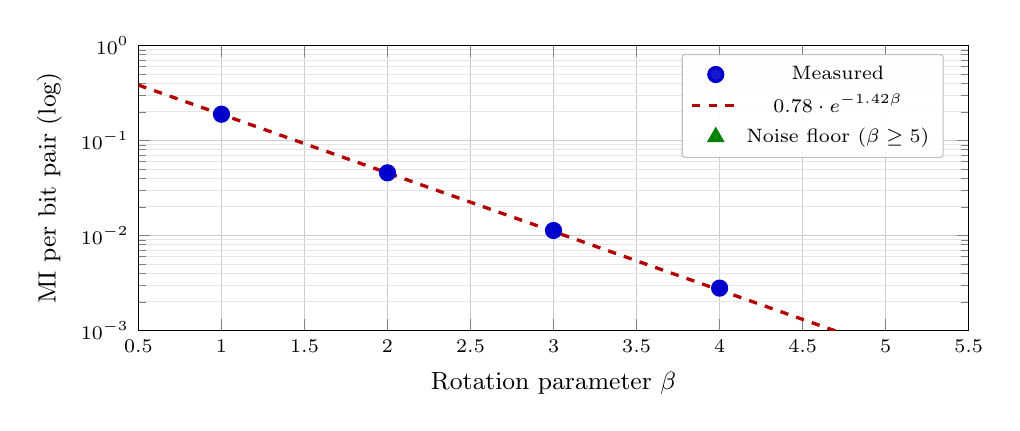
\begin{tikzpicture}
\begin{semilogyaxis}[
    width=\columnwidth,
    height=5.2cm,
    xlabel={Rotation parameter $\beta$},
    ylabel={MI per bit pair (log)},
    grid=both,
    grid style={gray!20},
    major grid style={gray!40},
    xmin=0.5, xmax=5.5,
    ymin=0.001, ymax=1,
    tick label style={font=\scriptsize},
    label style={font=\small},
    legend style={font=\scriptsize, at={(0.97,0.97)}, anchor=north east, draw=gray!50, fill=white, fill opacity=0.9, text opacity=1, rounded corners=1pt},
    every axis plot/.append style={very thick},
]
\addplot[blue!80!black, mark=*, mark size=2.5pt, only marks] coordinates {(1,0.189045)(2,0.045687)(3,0.011291)(4,0.002792)};
\addplot[red!70!black, domain=0.5:5.5, samples=80, dashed] {0.78*exp(-1.42*x)};
\addplot[green!50!black, mark=triangle*, mark size=2.5pt, only marks] coordinates {(5,0.00067)};
\legend{Measured, $0.78 \cdot e^{-1.42\beta}$, Noise floor ($\beta \geq 5$)}
\end{semilogyaxis}
\end{tikzpicture}
\caption{Leak-rate formula validation. Measured MI (blue dots) versus prediction (dashed red). At $\beta \geq 5$ the signal vanishes into noise (green triangle). The formula is independent of word size~WS and position parameter~$\alpha$.}
\label{fig:formula}
\end{figure}

\begin{table}[t]
\centering
\caption{Formula validation: measured vs.\ predicted MI per bit pair.}
\label{tab:formula}
\begin{tabular}{@{}cccr@{}}
\toprule
$\beta$ & \textbf{Measured} & \textbf{Predicted} & \textbf{Error} \\
\midrule
1 & 0.189045 & 0.189031 &  0.0\% \\
2 & 0.045687 & 0.045800 &  0.2\% \\
3 & 0.011291 & 0.011097 &  1.7\% \\
4 & 0.002792 & 0.002689 &  3.7\% \\
$\geq$5 & 0.000000 & --- & Noise \\
\bottomrule
\end{tabular}
\end{table}

Key properties of (\ref{eq:formula}): (i)~MI is independent of the word size~WS (verified at WS\,=\,16, 24, 32, 64---all yield MI\,$=$\,0.011 at $\beta{=}3$); (ii)~the universal death threshold is $\beta \geq 5$, independent of WS; (iii)~the formula enables prediction of leakage from design parameters alone, without executing the cipher.

\subsection{Per-Variant Quantification}

Table~\ref{tab:variants} quantifies the leakage per round for all affected Speck variants using (\ref{eq:formula}).

\begin{table}[t]
\centering
\caption{Per-variant leak quantification from~(\ref{eq:formula}).}
\label{tab:variants}
\begin{tabular}{@{}lccccr@{}}
\toprule
\textbf{Variant} & $\alpha/\beta$ & \textbf{Active} & \textbf{MI/pair} & \textbf{Total} & \textbf{\%} \\
\midrule
Speck 32/64   & 7/2 & 14/16 & 0.046 & 0.64\,b & 4.0 \\
Speck 48/96   & 8/3 & 21/24 & 0.011 & 0.24\,b & 1.0 \\
Speck 64/128  & 8/3 & 29/32 & 0.011 & 0.33\,b & 1.0 \\
Speck 128/256 & 8/3 & 61/64 & 0.011 & 0.69\,b & 1.1 \\
\bottomrule
\end{tabular}
\end{table}

\section{Topological Classification}

\subsection{Necessary and Sufficient Condition}

Through systematic evaluation of six distinct operation orderings at WS\,=\,16 with $R{=}15$ (Table~\ref{tab:topology}), we establish:

\textit{F8 leakage exists if and only if the modular addition output enters the cipher state without prior diffusion that destroys the carry-chain correlation.}

\begin{table}[t]
\centering
\caption{Topology sweep (WS\,=\,16, $R{=}15$). Only two orderings produce persistent leakage. $Z$ values at three $\beta$ settings.}
\label{tab:topology}
\begin{tabular}{@{}lrrrl@{}}
\toprule
\textbf{Topology} & $\beta{=}1$ & $\beta{=}2$ & $\beta{=}5$ & \textbf{Leak?} \\
\midrule
\textbf{ROR$\to$ADD$\to$XOR (Speck)} & 12,745 & 3,436 & 42 & \textbf{Yes} \\
ROT$\to$ADD$\to$XOR & 1.9 & 2.3 & 2.4 & No \\
ADD$\to$XOR$\to$ROT & 3.0 & 2.3 & 1.9 & No \\
XOR$\to$ADD$\to$ROT & 2.8 & 1.9 & 2.6 & No \\
Bare ADD (no rotation) & 71,946 & 71,946 & 71,946 & Yes \\
\textbf{Threefish MIX} & 14,513 & 3,030 & 38 & \textbf{Yes} \\
\bottomrule
\end{tabular}
\end{table}

\subsection{Two Distinct Mechanisms}

\textbf{$\beta$-Masking (Speck family):} The Speck round function computes $x' = (\mathrm{ROR}(x, \alpha) + y) \oplus k$, $y' = \mathrm{ROL}(y, \beta) \oplus x'$. The rotation $\mathrm{ROL}(y, \beta)$ masks the lower $\beta$~bits of the XOR with~$x'$, while the remaining $\mathrm{WS}{-}\beta$ bits retain carry-chain correlation. The signal lies on the $(\alpha{+}\beta)$-shifted diagonal.

\textbf{Raw Carry (Threefish):} The Threefish MIX function computes $e_0 = x_0 + x_1$, $e_1 = \mathrm{ROL}(x_1, R) \oplus e_0$. The rotation acts on the XOR operand, not on the addition output. The low bits of $e_0$ directly expose the carry chain (effective $\beta_{\mathrm{eff}} = 0$), with MI decaying from 0.9999 at bit~0 to noise at bit~5.

\section{Comparison with Prior Art}

\subsection{Gohr's Neural Distinguisher}

Table~\ref{tab:gohr} compares F8 with Gohr's~\cite{gohr2019} residual neural network on Speck~32/64.

\begin{table}[t]
\centering
\caption{F8 vs.\ Gohr~\cite{gohr2019} on Speck~32/64. F8 detects at all rounds; Gohr's differential trail decays to chance at R6.}
\label{tab:gohr}
\begin{tabular}{@{}rrll@{}}
\toprule
\textbf{Rounds} & \textbf{F8 $Z$} & \textbf{Gohr Acc.} & \textbf{Detects} \\
\midrule
R5  & $+$7,000+ & 71.7\%   & Both \\
R6  & $+$7,000+ & $\sim$50\% & F8 only \\
R7  & $+$7,000+ & $\sim$50\% & F8 only \\
R8+ & $+$7,000+ & $\sim$50\% & F8 only \\
\bottomrule
\end{tabular}
\end{table}

\begin{figure}[t]
\centering
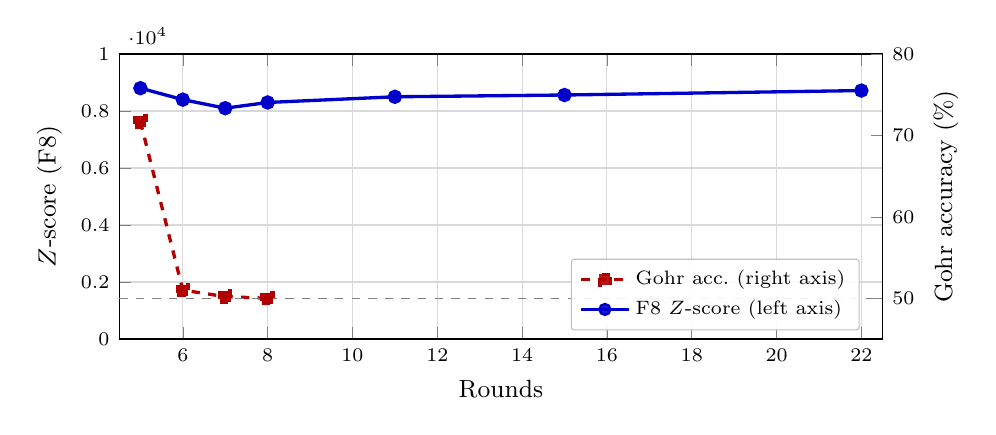
\begin{tikzpicture}
\begin{axis}[
    width=0.93\columnwidth,
    height=5.2cm,
    xlabel={Rounds},
    ylabel={$Z$-score (F8)},
    axis y line*=left,
    ymin=0, ymax=10000,
    xmin=4.5, xmax=22.5,
    grid=both,
    grid style={gray!15},
    major grid style={gray!30},
    tick label style={font=\scriptsize},
    label style={font=\small},
    every axis plot/.append style={very thick},
]
\addplot[blue!80!black, mark=*, mark size=2pt] coordinates {(5,8802)(6,8400)(7,8100)(8,8300)(11,8500)(15,8562)(22,8718)};
\end{axis}
\begin{axis}[
    width=0.93\columnwidth,
    height=5.2cm,
    axis y line*=right,
    axis x line=none,
    ylabel={Gohr accuracy (\%)},
    ymin=45, ymax=80,
    xmin=4.5, xmax=22.5,
    tick label style={font=\scriptsize},
    label style={font=\small},
    every axis plot/.append style={very thick},
    legend style={font=\scriptsize, at={(0.97,0.03)}, anchor=south east, draw=gray!50, fill=white, fill opacity=0.9, text opacity=1, rounded corners=1pt, cells={anchor=west}},
]
\addplot[red!70!black, mark=square*, mark size=2pt, dashed] coordinates {(5,71.7)(6,51)(7,50.2)(8,50)};
\addlegendentry{Gohr acc.\ (right axis)}
\addlegendimage{blue!80!black, mark=*, mark size=2pt, thick}
\addlegendentry{F8 $Z$-score (left axis)}
\draw[gray, dashed, thin] (axis cs:4.5,50) -- (axis cs:22.5,50);
\end{axis}
\end{tikzpicture}
\caption{F8 (blue) vs.\ Gohr neural distinguisher (red dashed) on Speck~32/64. Gohr decays to 50\% at R6; F8 remains at $Z > +8{,}000$ through all 22~rounds.}
\label{fig:gohr}
\end{figure}

The methods detect fundamentally different phenomena (Fig.~\ref{fig:gohr}). Gohr's network learns chosen-plaintext differential trails that decay exponentially with round count. F8 detects same-key cross-round carry correlations that are regenerated per round. The convergence at R5 (both detect) and divergence from R6 (F8 only) directly reflects this distinction: differential trails through 6+ Speck rounds decay below the neural network's detection threshold, while the per-round carry leak is stationary.

\subsection{Relation to CASI and Crypto-CASI}

Our prior work introduced CASI~\cite{foss2026crypto} for single-round security margin analysis and Crypto-CASI~\cite{foss2026artifact} for black-box PQC characterization. Both operate on output from a \emph{single} round configuration. F8 extends this framework to \emph{cross-round} analysis, targeting a leakage class invisible to single-round metrics: the statistical dependency between consecutive round outputs. CASI correctly identifies Speck as secure at full rounds (CASI\,$\approx$\,1.0 from R7), because single-round output is well-diffused. F8 reveals that the \emph{relationship between} consecutive rounds retains structure---a complementary and independent finding.

\subsection{Universal Leak-Model Compiler}

A three-rule hierarchical compiler maps cipher specifications to leak profiles:

\begin{enumerate}[nosep]
\item \textbf{Inter-round diffusion layer} $\to$ Secure (SPARX: linear layer eliminates leakage completely).
\item \textbf{$\geq$2 additions per word + cross-mixing} $\to$ Secure (Chaskey, LEA, HIGHT: intra-round diffusion kills signal within 2--3 rounds).
\item \textbf{Topology check}: Only ROR$\to$ADD$\to$XOR (Speck) and ADD$\to$ROT\textsubscript{other}$\to$XOR (Threefish MIX) are vulnerable. All other orderings yield $Z \approx 0$.
\end{enumerate}

Validated against 9~configurations (8~cipher families plus SPARX ARX-box in isolation) with 100\% accuracy (Table~\ref{tab:compiler}).

\begin{table}[t]
\centering
\caption{Leak-model compiler validation: 9/9 correct predictions (including SPARX ARX-box in isolation).}
\label{tab:compiler}
\begin{tabular}{@{}llll@{}}
\toprule
\textbf{Cipher} & \textbf{Predicted} & \textbf{Empirical} & \textbf{Match} \\
\midrule
Speck 32/64    & Vuln ($\beta$-mask) & $Z \approx 8{,}000$ & \checkmark \\
Speck 64/128   & Vuln ($\beta$-mask) & $Z \approx 5{,}000$ & \checkmark \\
Speck 128/256  & Vuln ($\beta$-mask) & $Z \approx 4{,}000$ & \checkmark \\
Threefish-256  & Vuln (raw carry)    & $Z \approx 5{,}900$ & \checkmark \\
SPARX-64/128   & Secure & $Z \approx 0$ & \checkmark \\
\rowcolor{orange!12} \quad\textit{ARX-box} & \textit{Vuln ($\beta$-mask)} & \textit{$Z \approx 5{,}500$} & \textit{\checkmark} \\
Chaskey        & Secure & $Z \approx 0$ & \checkmark \\
LEA-128        & Secure & $Z \approx 0$ & \checkmark \\
HIGHT          & Secure & $Z \approx 0$ & \checkmark \\
\bottomrule
\end{tabular}
\end{table}

\section{Discussion}

\subsection{Cryptographic Implications}

For \textbf{Speck}, F8 yields full-round known-key distinguishers for the entire family. The effective security margin in the known-key model is reduced to zero---not because the cipher has too few rounds, but because the leakage is per-round stationary. Practical impact for standard encryption is limited (known-key setting), but the theoretical significance is considerable.

For \textbf{Threefish-256/Skein}, the known-key model is the \emph{operationally relevant} model: the hash function's compression function treats the message block as a key. A $Z \approx +5{,}900$ distinguisher at all 72~rounds is directly relevant to Skein's security claim.

For \textbf{SPARX}, the linear inter-round layer is the sole protection mechanism. The ARX-box in isolation produces $Z \approx +5{,}500$ with MI\,$=$\,0.640---identical to pure Speck (Table~\ref{tab:immunity}). Algebraic inversion of the linear layer fails to recover the signal ($Z < 1.5$). This validates SPARX's design philosophy: the mixing layer is not merely beneficial for diffusion---it is \emph{essential} for eliminating carry-chain leakage that the ARX primitive alone cannot prevent.

\subsection{Comparison with Existing Methods}

Table~\ref{tab:prior-art} summarizes the key distinctions between F8 and established cryptanalytic methods.

\begin{table}[t]
\centering
\caption{F8 versus established methods. F8 is the only method detecting non-decaying, per-round regenerated leakage.}
\label{tab:prior-art}
\small
\begin{tabular}{@{}lllll@{}}
\toprule
\textbf{Method} & \textbf{Signal} & \textbf{Max R} & \textbf{Cost} & \textbf{Univ.} \\
\midrule
Differential~\cite{biham1991} & Decays & Limited & Manual & No \\
Linear~\cite{matsui1993} & Decays & Limited & Manual & No \\
Rotational~\cite{khovratovich2010} & Decays & Limited & Manual & No \\
Neural~\cite{gohr2019} & Decays & R7--8 & GPU & No \\
Known-key~\cite{knudsen2007} & Decays & 7R AES & Manual & No \\
\midrule
\textbf{F8 (this work)} & \textbf{Station.} & \textbf{All R} & \textbf{CPU} & \textbf{Yes} \\
\bottomrule
\end{tabular}
\end{table}

\subsection{Computational Cost}

F8 analysis of a single cipher configuration requires $N = 10^5$ samples and $K = 20$ permutations, completing in under 10~seconds on a single CPU core. The entire 13-cipher survey completes in under 3~minutes. By comparison, Gohr's neural distinguisher requires $10^7$ training samples, GPU computation, and hours of training per cipher---and must be retrained for each new cipher family. The leak-model compiler evaluates a cipher specification in milliseconds, requiring no cipher execution at all.

\subsection{Design Guidance}

The topological classification yields concrete design rules for new ARX constructions: (i)~ensure addition outputs pass through a diffusion layer before entering the state; (ii)~use $\beta \geq 5$ if a single rotation must serve as the only diffusion mechanism; (iii)~employ inter-round mixing layers (SPARX approach); or (iv)~use $\geq$2 additions per word with cross-element mixing (Chaskey/LEA approach).

\subsection{Limitations}

F8 operates in the known-key model and does not imply practical key-recovery attacks on ciphertext encrypted with unknown keys. The test requires configurable round-count access to the cipher implementation. The prediction formula (\ref{eq:formula}) is validated for $\beta \in \{1, 2, 3, 4\}$; extrapolation beyond $\beta = 4$ is bounded by the noise floor. The compiler is validated on 9~configurations; additional architectures (e.g., PRESENT, Camellia) require separate evaluation. Whether the carry-chain leakage can be amplified into a distinguishing advantage in a standard (unknown-key) attack model remains an open question.

\subsection{Reproducibility}

All experiments are implemented in the \texttt{live-casi} Python package~\cite{livecasi} available on PyPI. The F8 module provides both informed and black-box modes, the prediction function, and the leak-model compiler with pre-validated cipher specifications for all 13~tested families.

\subsection{Open Questions}

Several directions remain for future investigation: (i)~Whether the known-key carry leakage can be amplified into a chosen-plaintext or ciphertext-only distinguishing advantage, which would elevate the finding from a theoretical observation to a practical attack. (ii)~Extension of the topology sweep to additional ARX cipher families beyond the 13~tested, particularly newer lightweight constructions submitted to NIST standardization processes. (iii)~Whether the Threefish raw-carry mechanism affects the collision resistance of Skein beyond the known-key distinguisher demonstrated here. (iv)~Application of the F8 framework to ARX-based authenticated encryption modes (e.g., NORX, SPARKLE) and to the modular arithmetic components of lattice-based post-quantum constructions, where modular addition over larger moduli may exhibit analogous carry-chain properties. (v)~Theoretical derivation of the prediction formula coefficients ($A = 0.78$, $B = 1.42$) from the probability theory of carry propagation in modular addition, which would place the currently empirical formula on a formal mathematical foundation.

\section{Conclusion}

F8 reveals a previously unknown class of structural leakage in ARX ciphers: persistent, per-round-regenerated carry-chain correlations that do not decay with additional rounds. The closed-form prediction function $\mathrm{MI}(\beta) = 0.78 \cdot \exp(-1.42\beta)$ enables evaluation from design parameters alone, without cipher execution. The topological classification provides a necessary and sufficient condition: leakage exists if and only if a modular addition output enters the cipher state without prior diffusion. Two distinct mechanisms---$\beta$-masking and raw carry exposure---account for all observed leakage patterns across 13~cipher families. The universal leak-model compiler translates these findings into an automated evaluation tool with 9/9 validated predictions.

Full-round known-key distinguishers for the entire Speck family (4~variants, $Z > +4{,}000$) and for Threefish-256 ($Z \approx +5{,}900$ at all 72~rounds) demonstrate that this leakage class affects widely deployed constructions. The SPARX ARX-box in isolation produces $Z \approx +5{,}500$ (identical to Speck), proving that the linear inter-round layer---not the ARX primitive---is the sole protection mechanism; algebraic inversion of this layer fails to recover the signal. Control experiments with SIMON~32/64 and a random Feistel cipher isolate modular addition as the necessary condition for F8 leakage. The strictly encrypt-only nature (ratio $> 3{,}000{:}1$), independence from key material, sample size, and round count, and the reduced-round analysis of four immune ciphers (all exhibiting carry-leakage at early rounds before diffusion eliminates it) collectively confirm that carry-chain correlation is a fundamental structural property of specific ARX topologies. All code and data are available via the open-source \texttt{live-casi} package~\cite{livecasi}.

\begin{thebibliography}{00}

\bibitem{biham1991} E. Biham and A. Shamir, ``Differential cryptanalysis of DES-like cryptosystems,'' \textit{J. Cryptology}, vol.~4, no.~1, pp. 3--72, 1991.

\bibitem{matsui1993} M. Matsui, ``Linear cryptanalysis method for DES cipher,'' in \textit{Proc. EUROCRYPT '93}, pp. 386--397, 1993.

\bibitem{gohr2019} A. Gohr, ``Improving attacks on round-reduced Speck32/64 using deep learning,'' in \textit{Proc. CRYPTO 2019}, pp. 150--179, 2019.

\bibitem{khovratovich2010} D. Khovratovich and I. Nikolić, ``Rotational cryptanalysis of ARX,'' in \textit{Proc. FSE 2010}, pp. 333--346, 2010.

\bibitem{ferguson2010} N. Ferguson et al., ``The Skein hash function family,'' Submission to NIST SHA-3 competition, 2010.

\bibitem{bernstein2008} D. J. Bernstein, ``ChaCha, a variant of Salsa20,'' in \textit{Workshop Record of SASC 2008}, 2008.

\bibitem{dinu2016} D. Dinu et al., ``Design strategies for ARX with provable bounds: Sparx and LAX,'' in \textit{Proc. ASIACRYPT 2016}, pp. 484--513, 2016.

\bibitem{foss2026crypto} D. T. Foss, ``Causal graph topology for automated security margin analysis and blind cipher identification,'' in \textit{Proc. ICECET 2026}, IEEE, to appear.

\bibitem{foss2026artifact} D. T. Foss, ``Compression isolation of distributional signatures in NIST post-quantum ciphertext,'' in \textit{Proc. ICECET 2026}, IEEE, to appear.

\bibitem{aumasson2014} J.-P. Aumasson et al., ``NORX: Parallel and scalable AEAD,'' in \textit{Proc. ESORICS 2014}, pp. 19--36, 2014.

\bibitem{daemen2002} J. Daemen and V. Rijmen, \textit{The Design of Rijndael: AES -- The Advanced Encryption Standard}. Springer, 2002.

\bibitem{biryukov2014} A. Biryukov and V. Velichkov, ``Automatic search for differential trails in ARX ciphers,'' in \textit{Proc. CT-RSA 2014}, pp. 227--250, 2014.

\bibitem{khovratovich2015} D. Khovratovich et al., ``Rotational-XOR cryptanalysis of reduced-round SPECK,'' IACR ePrint 2015/1065, 2015.

\bibitem{benamira2021} A. Benamira et al., ``A deeper look at machine learning-based cryptanalysis,'' in \textit{Proc. EUROCRYPT 2021}, pp. 805--835, 2021.

\bibitem{knudsen2007} L. R. Knudsen and V. Rijmen, ``Known-key distinguishers for some block ciphers,'' in \textit{Proc. ASIACRYPT 2007}, pp. 315--324, 2007.

\bibitem{livecasi} D. T. Foss, ``live-casi: Black-box cipher analysis tool,'' PyPI, 2026, \url{https://pypi.org/project/live-casi/}.

\end{thebibliography}

\end{document}
